\documentclass{beamer}
\usepackage{chemformula}
\usepackage{hyperref}
\usepackage{graphicx,caption}
\usepackage[mediumspace,mediumqspace,squaren]{SIunits}
\usetheme{Madrid}
\title[Two Dimensional Materials]{Two Dimensional Material, Their Properties, Application and Manufacturing}
\subtitle{Reading Assignment}
\author{Shibu Meher}
\institute{IIT Bhubaneswar}
\date{\today}

\begin{document}

\begin{frame}
\titlepage
\end{frame}

\begin{frame}
\frametitle{Outline}
\tableofcontents
\end{frame}

\section{Introduction}

\begin{frame}{Foundation of Technology}
    \begin{itemize}
        \item How well we understand material system
        \item Material properties depends on what it is made up
        \item Does the properties depend on size?
    \end{itemize}
    \begin{figure}
        \centering
        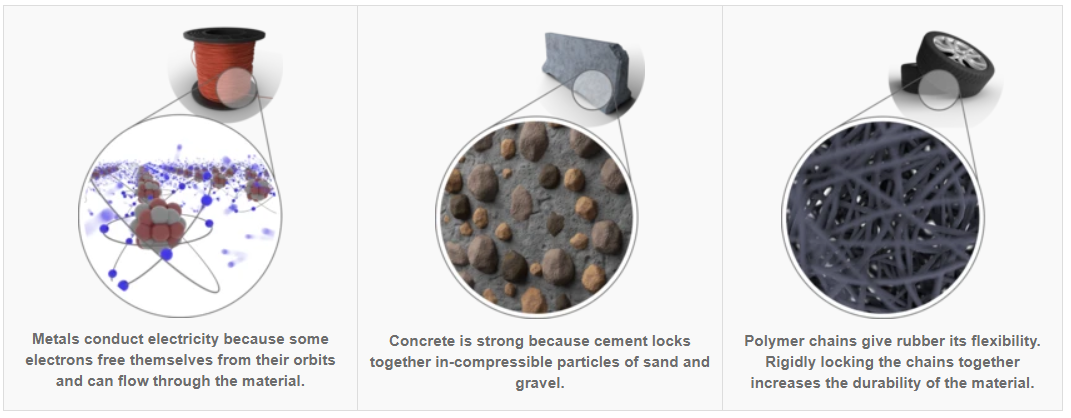
\includegraphics[scale=0.5]{copper_concrete_rubber.PNG}
    \end{figure}
\end{frame}

\section{What are 2D materials?}

\begin{frame}
\frametitle{Nanomaterials}
\begin{itemize}
    %\setlength\itemsep{2em}
    \item Having at least one dimension in nano-scale ($< 100 nm$)
    \item Materials - 
    \begin{itemize}
        \item $0D$ Material - nanoparticle, e.g. quantum dots
        \item $1D$ Material - nanotube/nanowire, e.g. carbon nanotube
        \item $2D$ Material - sheet or film with thickness in nano-scale, e.g. graphene
        \item $3D$ Material or Bulk material - e.g. block of iron.
    \end{itemize}
\end{itemize}
\begin{figure}
    \centering
    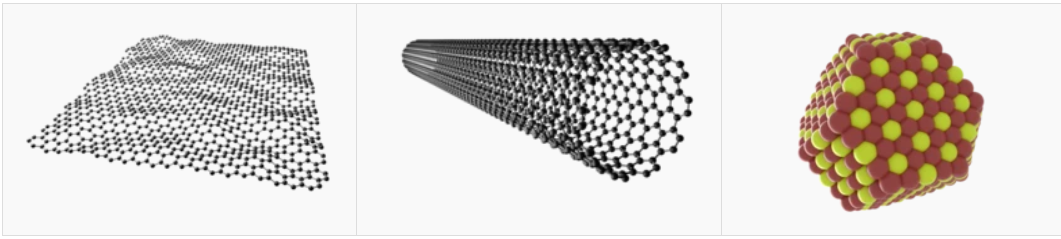
\includegraphics[scale=0.5]{nanomaterial.PNG}
\end{figure}

\end{frame}

\begin{frame}{Properties and example of 2D Material}
    \begin{itemize}
    \setlength\itemsep{2em}
    \item Due to nanoscale dimension following properties are affected.
    \begin{itemize}
        \item Electrical and thermal conductivity
        \item Chemical reactivity
        \item Mechanical properties
        \item Interaction with light and other radiation and beam of particle
        \item New phenomenon - Quantum hall effect, Berry phase
    \end{itemize}
    \item Example - Graphene, Hexagonal Boron Nitride (h-BN), Transition Metal Di-Chalcogenides(TMDCs), Phosphorene, Xenes etc.
\end{itemize}
\end{frame}

\begin{frame}{Graphene and h-BN}
    \begin{figure}
        \centering
        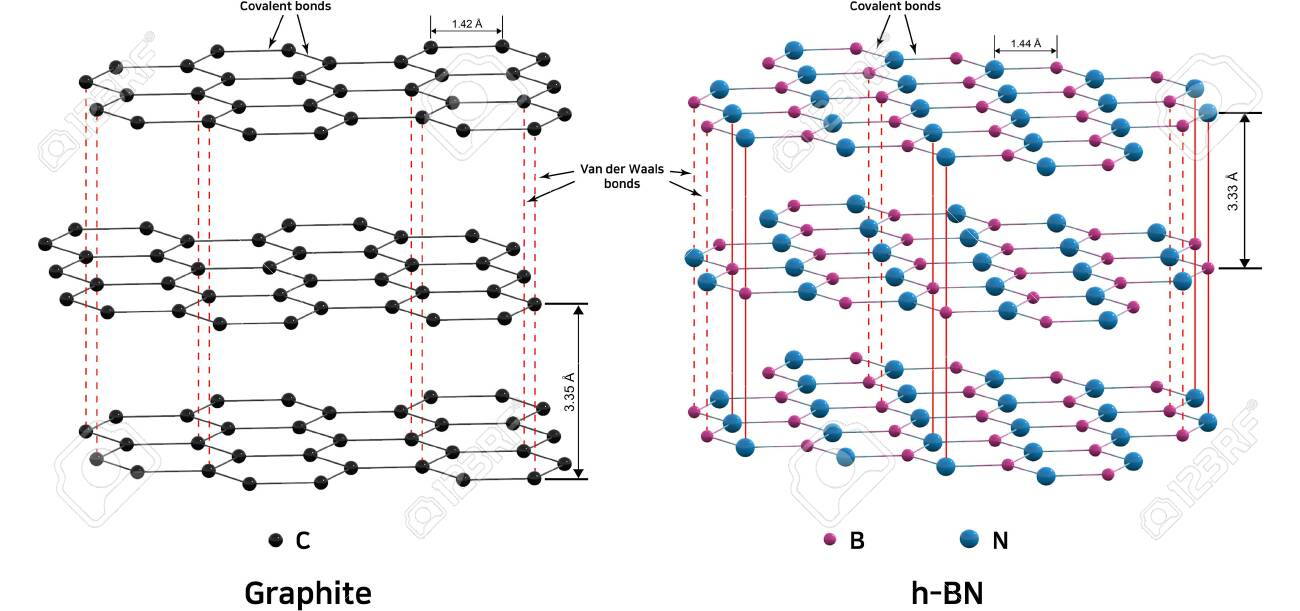
\includegraphics{133940929-hexagonal-boron-nitride-and-carbon-graphite-crystalline-structure.jpg}
    \end{figure}
\end{frame}

\begin{frame}{Graphene}
\begin{itemize}
\setlength\itemsep{1em}
    \item Covalently bonded hexagonal lattice of carbon
    \item One atom thick - $0.14 nm$
    \item Semimetal - Valance and conduction band touch each other
    \item Unique band structure - Extremely high speed of electron($\frac{1}{300}$ the speed of light) leading to exceptional thermal conductivity
    \item Has highest tensile strength
    \item Fascinating Physical phenomenon - Quantum hall effect, Berry phase
\end{itemize}
\end{frame}

\begin{frame}{h-BN}
    \begin{itemize}
        \item Has same crystallographic appearance as graphene except that it has B and N atom
        \item Wide band gap insulator
    \end{itemize}
    \begin{figure}
        \centering
        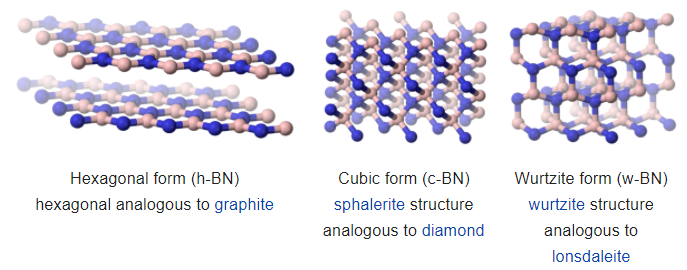
\includegraphics[scale=0.7]{h-BN.PNG}
    \end{figure}
\end{frame}

\begin{frame}{Transition Metal Dichalcogenides or TMDCs or $MX_2$}
\begin{itemize}
    \item M - Metal atom, e.g. Mo, W
    \item X - Chalcogens/oxygen family, e.g. S, Se, Te
    \item van der Waals material - layer material
    \item Metal layer is sandwiched between chalcogenide layer
    \item Two phases - 2H phase (triagonal, semiconductor, e.g. $MoS_2$, $WS_2$, $MoSe_2$) and 1T phase (hexagonal, metallic, e.g. $WTe_2$)
\end{itemize}
\begin{figure}
    \centering
    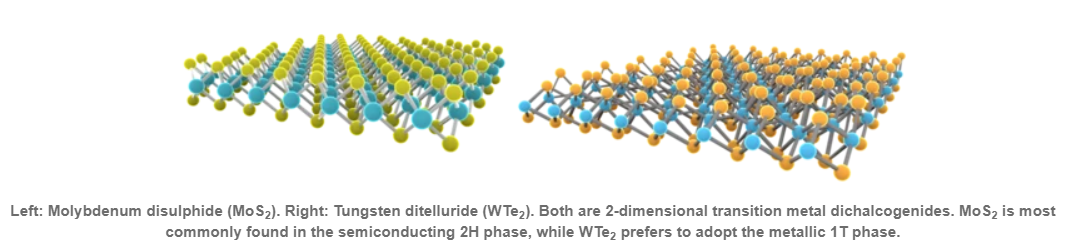
\includegraphics[scale=0.5]{TMDCs.PNG}
\end{figure}
\end{frame}

\begin{frame}{Direct and Indirect Band gap}
\begin{itemize}
    \item 2H phase - indirect band gap in bulk and direct band gap in monolayer - suitable for optoelectronics
    \item Direct and Indirect band gap
\end{itemize}
\begin{columns}
    \column{0.5\textwidth}
    \begin{figure}
        \centering
        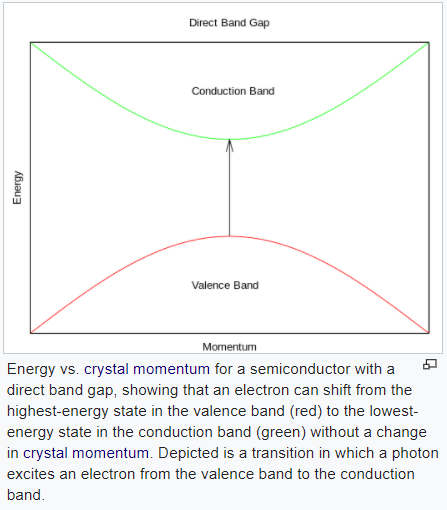
\includegraphics[scale=0.5]{direct.PNG}
    \end{figure}
    \column{0.5\textwidth}
    \begin{figure}
        \centering
        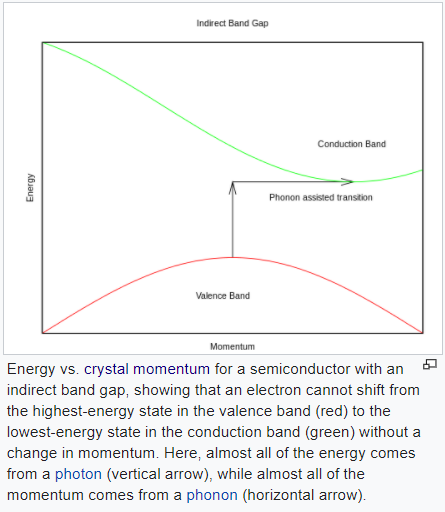
\includegraphics[scale=0.5]{indirect.PNG}
    \end{figure}
    
\end{columns}
\end{frame}

\begin{frame}{Phosphorene}
    \begin{itemize}
        \item Direct band gap semiconductor
        \item Wrinkled honey comb structure
        \item Band gap - tunable by stacking layers
        \item Good charge mobility - about $1000 \frac{cm^2}{Vs}$
        \item Anisotropic
        \item Application - Optoelectronics and transistors
    \end{itemize}
    \begin{figure}
        \centering
        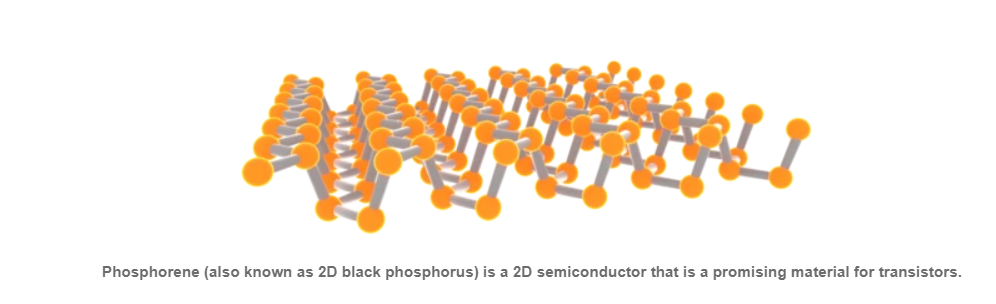
\includegraphics[scale=0.5]{phosphorene.PNG}
    \end{figure}
\end{frame}

\begin{frame}{Xenes}
    \begin{itemize}
        \item Monolayer of silicon(silicene), germanium(germanene), tin(stanene)
        \item Buckled hexagonal structure
        \item Can not be exfoliated, only grown epitaxially on substrate
        \item Have strong interaction with the substrate
        \item Recent - antimonene, bismuthine (magneto-electronics)
        \item Potential Application - Field Effect Transistors, topological insulator
    \end{itemize}
    \begin{figure}
        \centering
        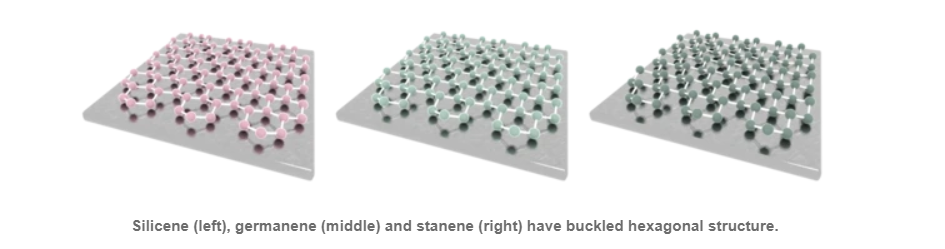
\includegraphics[scale=0.5]{xenes.PNG}
    \end{figure}
\end{frame}

% Section 3
\section{Why are 2D materials different from bulk materials?}

\begin{frame}{Why are 2D material different from bulk materials?}
    \begin{itemize}
        \item Removal of van der Waal interaction
    \end{itemize}
    \begin{figure}
        \centering
        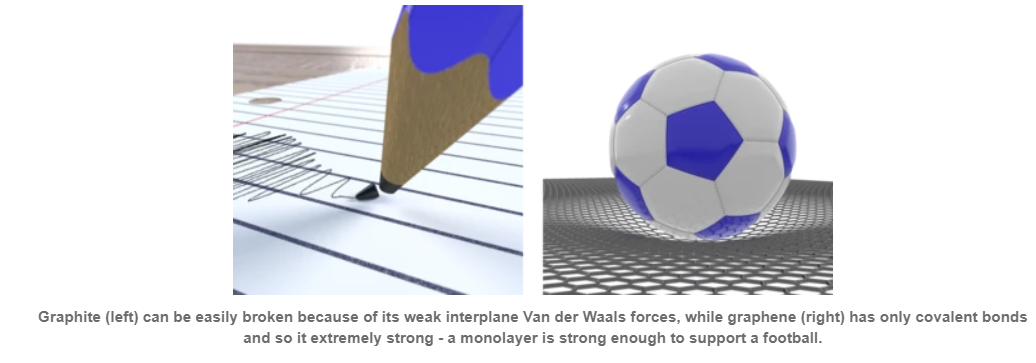
\includegraphics[scale=0.5]{removal_of_van_der_Waal.PNG}
    \end{figure}
\end{frame}

\begin{frame}{Why are 2D material different from bulk materials?}
    \begin{itemize}
        \item An increase in ratio of surface area to volume
        \begin{itemize}
            \item 2D material are more reactive than their bulk counterpart
            \item Suitable for sensing application
        \end{itemize}
    \end{itemize}
    \begin{figure}
        \centering
        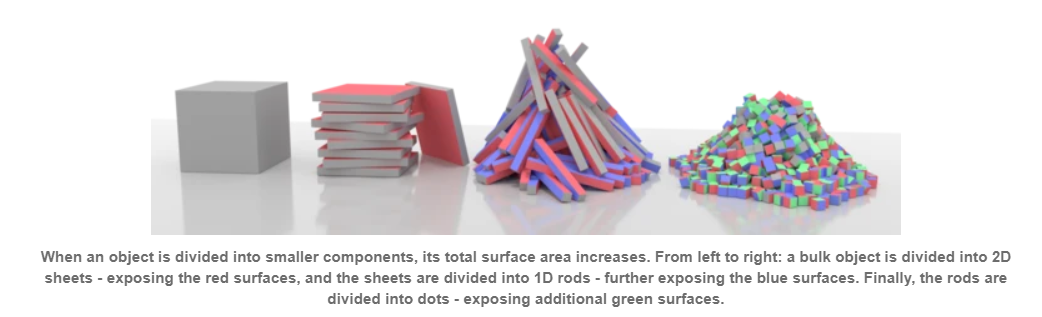
\includegraphics[scale=0.5]{increase_in_surface_area.PNG}
    \end{figure}
\end{frame}

\begin{frame}{Why are 2D material different from bulk materials?}
    \begin{itemize}
        \item Confinement of electrons in a plane
        \begin{itemize}
            \item Change in band structure - Indirect to direct
            \item Increase in band gap - Q. Why does the conductivity increases in case of graphene but not in case of h-BN?
        \end{itemize}
    \end{itemize}
    
    \begin{figure}
        \centering
        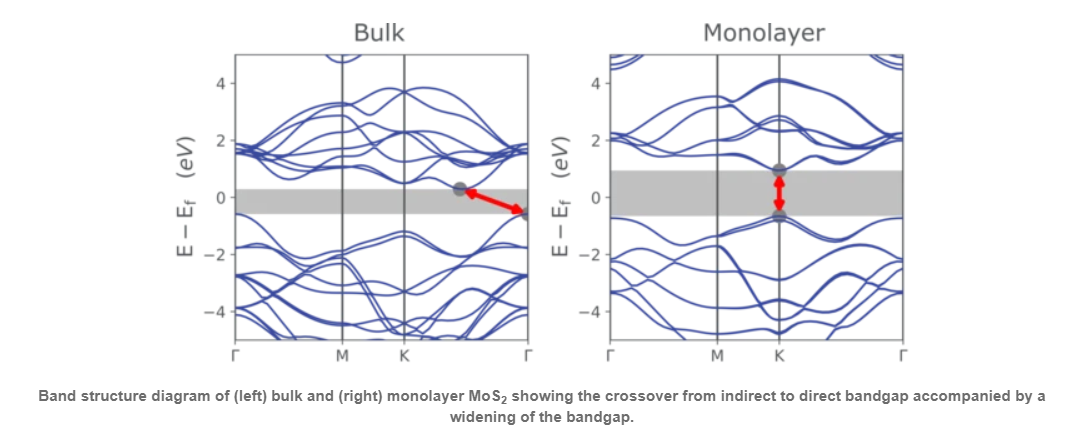
\includegraphics[scale=0.5]{confinement.PNG}
    \end{figure}
\end{frame}

\begin{frame}{Quantum Confinement}
    \begin{itemize}
        \item Increase in band gap
        \item Bohr radius
    \end{itemize}
    \begin{figure}
        \centering
        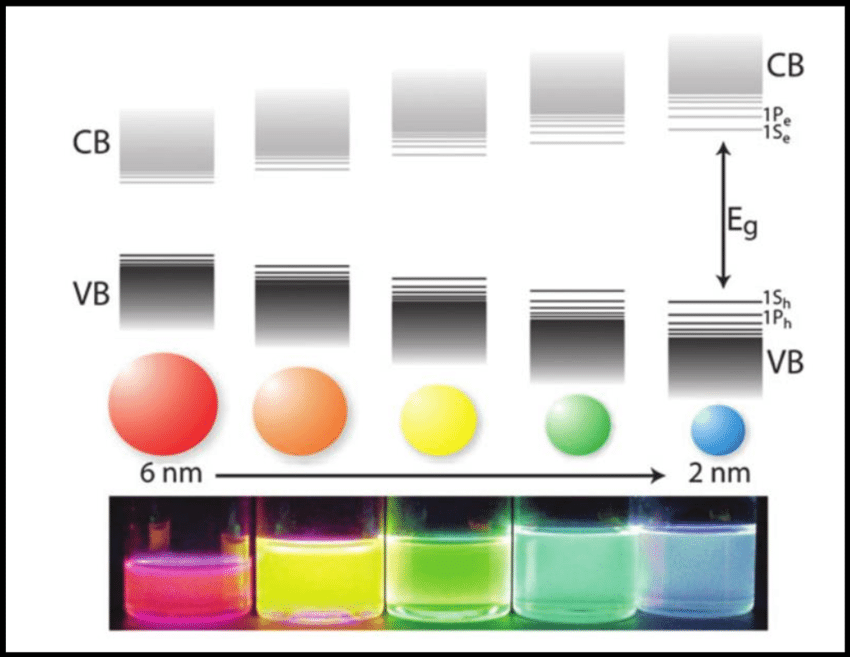
\includegraphics[scale = 0.3]{Quantum Confinement.png}
    \end{figure}
\end{frame}

% Section 4

\section{How to make 2D materials?}

\begin{frame}{Making of 2D Materials}
    \begin{itemize}
    \setlength\itemsep{2em}
        \item Graphene - First 2D material, 2004, Scotch-tap mechanical exfoliation
        \item van der Waals Material - Layered material
        \item Two approaches
        \begin{itemize}
            \item Top-down Approach - Start with bulk material make it thinner, e.g. Mechanical exfoliation, Liquid exfoliation
            \item Bottom-up Approach - Start with atomic ingredients and assemble them together, e.g. Chemical Vapour Deposition, Solution based chemical synthesis
        \end{itemize}
    \end{itemize}
\end{frame}

\begin{frame}{Top-down Approach}
    \begin{figure}
        \centering
        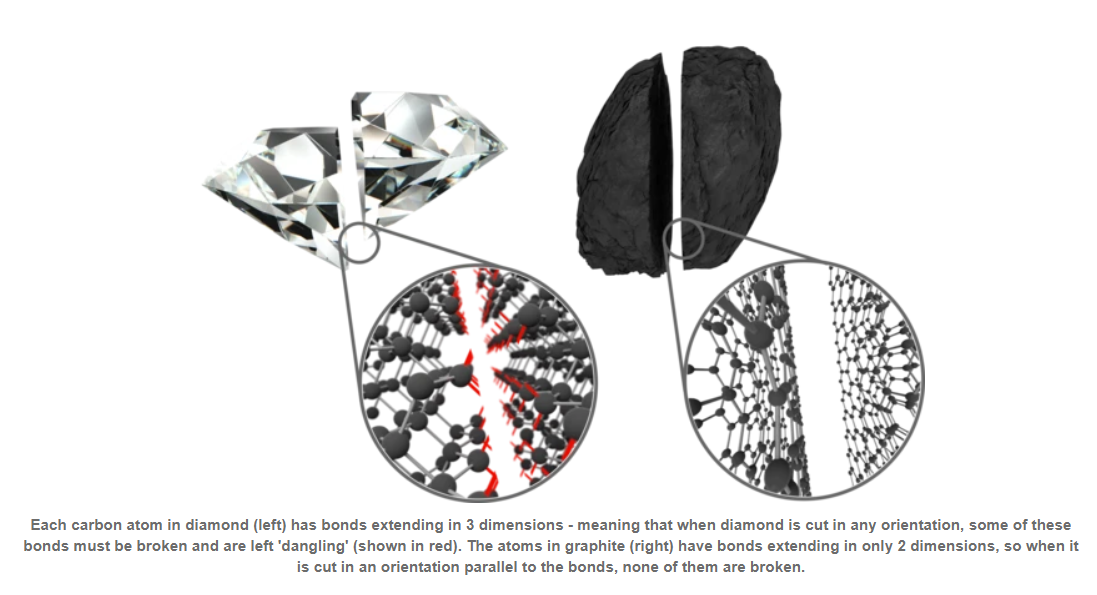
\includegraphics[scale=0.5]{breaking_bond.PNG}
    \end{figure}
\end{frame}

\begin{frame}{Mechanical Exfoliation or Scotch Tap Method}
    \begin{itemize}
        \item Monolayer yield is low
        \item No control of size and shape
        \item Size - reasonable - few microns to 100 microns
        \item Quality - excellent
        \item Popular for van der Waals material and lab based studies
    \end{itemize}
    \begin{figure}
        \centering
        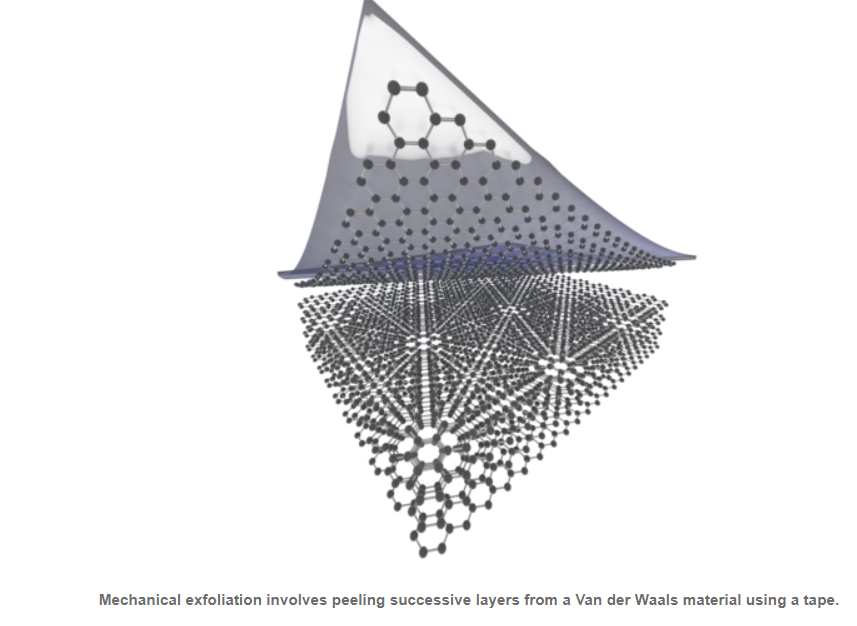
\includegraphics[scale = 0.4]{mechanical_exfoliation.PNG}
    \end{figure}
\end{frame}

\begin{frame}{Liquid Exfoliation}
    \begin{itemize}
        \item Use of organic solvent to create force between layer
        \item Sonication, Use of reactive ions
        \item Highly scalable
        \item Low monolayer yield, small flake size ($<100 nm$)
        \item Not suitable for optoelectronic application - high density of defects, residual solvent
    \end{itemize}
    \begin{figure}
        \centering
        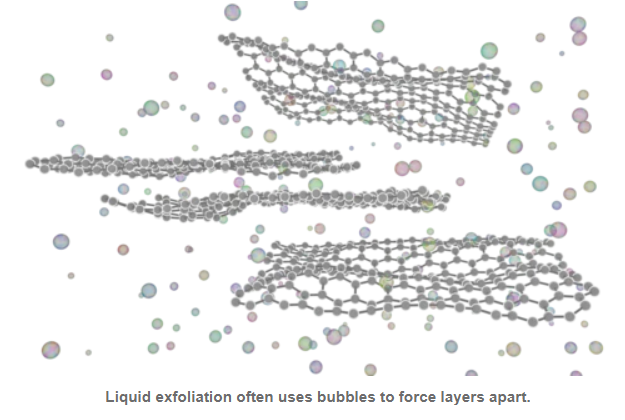
\includegraphics[scale = 0.5]{liquid_exfoliation.PNG}
    \end{figure}
\end{frame}

\begin{frame}{Chemical Vapour Deposition (CVD)}
    \begin{itemize}
        \item One or more precursor gases (containing ingredients for the film) are passed through a heated chamber where they react with each other or with the substrate to form thin layer of required material.
        \item Successfully applied - Graphene, TMDCs
        \item Complex and expensive
        \item Highly scalable and quality approaches that of mechanical exfoliation
        \item Similar bottom up approaches - Physical Vapour Deposition (PVD), Vapour Phase Transport (VPT), Molecular Assembly, Atomic Layer Deposition
    \end{itemize}
\end{frame}


\section{Application of 2D materials}

\begin{frame}{Application of 2D materials}
    \begin{itemize}
    \setlength\itemsep{2em}
        \item Transistors and sensors
        \item Photodetectors
        \item Battery electrodes
        \item Topological insulators
        \item Valleytronics
    \end{itemize}
\end{frame}

\begin{frame}{2D Materials and Their Heterostructures}
    \begin{itemize}
        \item Extensive research - tunability, exotic properties of heterostructure
        \item Need - Method to produce scalable 2D materials and their heterostructure of high quality and low cost
        \item High Quality - Large area continuous 2D materials with uniform properties with low defect and less grain boundaries
        \item Example of suitable method - Chemical Vapour Deposition
    \end{itemize}
\end{frame}

\section{Chemical Vapour Deposition (CVD)}

\begin{frame}{Material Properties and CVD Parameters}
    \begin{itemize}
        \item Materials Features - Size of film, number of layers, morphology, orientation, phases, doping, defects, grain boundaries
        \item CVD Parameters - Temperature of the source zone and reactor zone, Chamber pressure, Carrier gas flow rate, partial pressure of source material in precursor gas, source substrate distance etc.
    \end{itemize}
    \begin{columns}
    \column{0.5\textwidth}
    \begin{figure}
        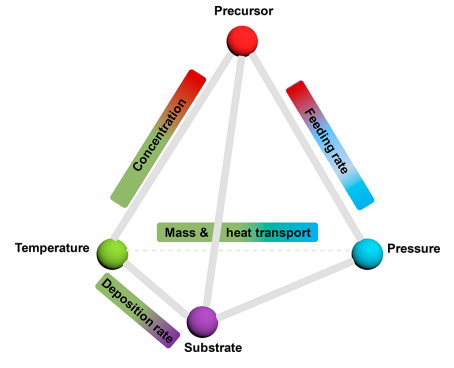
\includegraphics[scale = 0.5]{parameters_CVD.PNG}
    \end{figure}
    \column{0.5\textwidth}
    \begin{figure}
        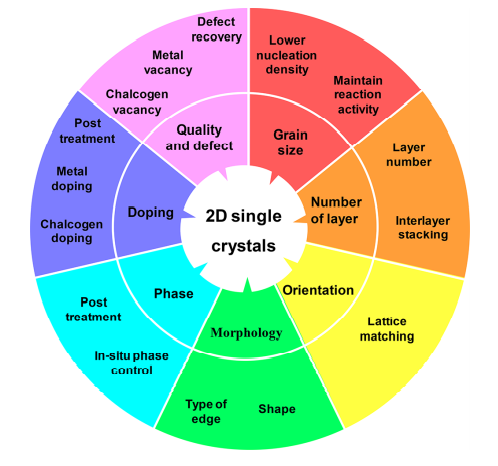
\includegraphics[scale = 0.5]{2D_material_features.PNG}
    \end{figure}
    \end{columns}
\end{frame}

\begin{frame}{CVD Parameters and their effect on Materials Properties}
    \begin{itemize}
        \item Precursor
        \item Temperature
        \item Substrate
        \item Pressure
        \item Modified CVD -- PECVD, ICP-CVD
    \end{itemize}
\end{frame}

\begin{frame}{Precursor}
    \begin{itemize}
        \item Reactant for CVD Process and Carrier gas
        \item Control the flow rate and partial pressure
        \item For Silicon growth
        \begin{itemize}
            \item Vapour Source - \ch{SiH4} or \ch{SiH2Cl2} gas (High Purity)
            \item Carrier Gas - \ch{H2} and \ch{Ar} - \ch{H2} terminates the dangling/broken bonds
        \end{itemize}
        \item For Graphen Growth
        \begin{itemize}
            \item Source Gas - \ch{CH4}
            \item Carrier Gas - \ch{H2}
            \item For Doping - \ch{NH3} or \ch{PH3}
        \end{itemize}
        \item For TMDCs growth
        \begin{itemize}
            \item Metal Source - Transition metal oxides (\ch{MoO3}, \ch{WO3}), Transition metal chlorides (\ch{MoCl5}), Metal foils
            \item Chalcogen source - \ch{S} or \ch{Se} powders
        \end{itemize}
    \end{itemize}
\end{frame}

\begin{frame}{Precursor}
    \begin{itemize}
        \item Problem - Very accurate temperature control in source zone - because vapour pressure of solid material is very sensitive to temperature
        \item Technology for TMDCs growth - Challenging, less mature
        \item Improved uniformity of TMDCs - \ch{Mo(CO)6}, \ch{CS(CH3)2} and \ch{H2S}
    \end{itemize}
\end{frame}

\begin{frame}{Temperature}
    \begin{itemize}
        \item Affect - flow of carrier gas, chemical reactions of precursors in the gas, deposition rate of product on the substrate
        \item Determines composition and uniformity of product
        \item High quality - High Temperature - High cost (Energy) - limited suitable substrate
        \item High Temperature - Enhances the mass transport, reaction rate and deposition rate.
        \item For TMDCs growth - Precise control of Temperature in source zone
    \end{itemize}
\end{frame}

\begin{frame}{Temperature}
    \begin{itemize}
        \item Two type of growth mechanisms of TMDCs
        \begin{itemize}
            \item Growth Controlled by chemical reaction rate - high temperature - high precursor concentration, high mass transport
            \item Mass transport limited growth mechanism - Low temperature - low precursor concentration, low mass transport
        \end{itemize}
        \item Gradient of precursor near substrate - Control is difficult
        \item Nucleation at vapour solid interface
        \begin{itemize}
            \item high temperature - Thermodynamic process
            \item low temperature - Kinetic process
        \end{itemize}
        \item For \ch{MoS2}, at $T > 800^{\circ}C$ - nucleation at the top of bottom layer - Control of number of layers
        \item High temperature - high growth rate - bigger size
    \end{itemize}
\end{frame}

\begin{frame}{Substrate}
    \begin{itemize}
        \item Substance over which 2D material nucleates and grows
        \item What makes a material good substrate for a particular 2D material growth?
        \item Multilayer and monolayer graphene growth - Catalytic active nickel and copper substrate - catalyst and substrate - reason - different carbon solubilities and catalytic activities
        \item TMDCs growth - intert \ch{Si}/\ch{SiO2}, mica and polyimide, gold or tungsten foil
        \item Nucleation and growth promoter of TMDCs - PTAS, PTCDA, rGO
        \item Additives to promote growth of TMDCs - alkali metal halides (\ch{NaCl}, \ch{KI}, \ch{KCl}, \ch{NaBr}, sodium cholate(\ch{C24H39NaO5}, \ch{NaOH})
    \end{itemize}
\end{frame}

\begin{frame}{Substrate}
    \begin{itemize}
        \item Growth promoter
        \begin{itemize}
            \item react with precursor (\ch{WO3}, \ch{MoO3}) to form volatile intermediate
            \item increase the domain size
            \item broaden the growth window (??)
            \item Opportunities - Function/mechanism are not clear.
        \end{itemize}
        \item Metal foil substrate
        \begin{itemize}
            \item gold crystallography - nucleation, domain size - reason - facet dependent binding energy between TMDCs and substrate
            \item Orentation - morphology e.g. \ch{MoS2} continuous film of domain size \unit{20}{\micro\meter} - vertical orientation - uniformity of precursur improved
        \end{itemize}
    \end{itemize}
\end{frame}

\begin{frame}{Substrate}
    \begin{itemize}
        \item Sapphire substrate
        \begin{itemize}
            \item $\alpha$-\ch{Al2O3} with trace amount of \ch{Fe}, \ch{Ti}, \ch{Cr}, \ch{V} or \ch{Mg}
            \item c-plane - specific orientation and atomically smooth surface terrace
            \item TMDCs grown - specific orientation - crystal symmetry and surface terrace of substrate
        \end{itemize}
    \begin{columns}
    \column{0.5\textwidth}
    \begin{figure}
        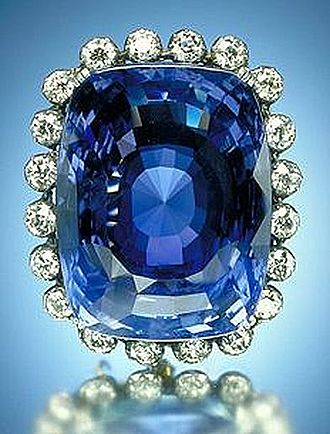
\includegraphics[scale = 0.3]{330px-Logan_Sapphire_SI.jpg}
    \end{figure}
    \column{0.5\textwidth}
    \begin{figure}
        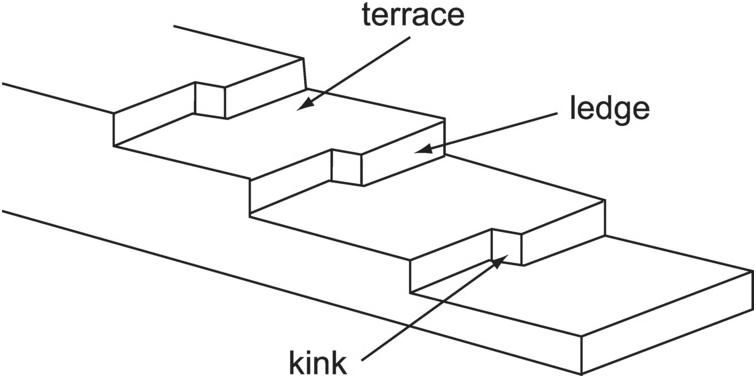
\includegraphics[scale = 0.7]{surface terrace.png}
    \end{figure}
    \end{columns}
    \end{itemize}
\end{frame}

\begin{frame}{Pressure}
    \begin{itemize}
        \item Varies from few atmospher to several millitor
        \item Influences gas flow behaviour e.g. at low pressure and same molar flow - high velocity of gas, high volume flow, precursor concentration decreased ( $PV = nRT$ ) - reaction more controllable (How?)
        \item low pressure CVD - Growth of wafer-scale continuous TMDC film
        \item Example - \ch{MoS2} growth - partial pressure of \ch{Mo(CO)6} is vital
        \begin{itemize}
            \item low pressure - nucleation only at grain boundaries
            \item high pressure - nucleation at the top of first layer (Multilayer product)
        \end{itemize}
    \end{itemize}
\end{frame}

\begin{frame}{Other Parameters of CVD}
    \begin{itemize}
        \item Thermal CVD - Thermal energy break the chemical bond of precursor molecule
        \item Other source of energy - plasma, light, laser - Modified CVD
        \item PECVD - Plasma Enhanced CVD
        \begin{itemize}
            \item Can conduct CVD of material for which Thermal CVD is not feasible
            \item Plasma - any gas where atoms or molecules are ionized into negatively charged electrons, positively charged ions and neutral species
            \item High energy of electrons - break precursor
            \item Interaction of surface and energetic ions - increase density of deposited film, remove contaminants, improve quality of film (How?)
            \item Example -- Conventional -- graphen on metal foil at $1000^{\circ}C$, Now graphene on glass without catalyst at $400-600^{\circ}C$ by PECVD
            \item PECVD \ch{MoS2} film -- precursor -- \ch{Mo} thin film and \ch{H2S} gas at $150-200^{\circ}C$
        \end{itemize}
    \end{itemize}
\end{frame}

\begin{frame}{Other Parameters of CVD}
    \begin{itemize}
        \item ICP-CVD -- Inductively Coupled CVD
        \begin{itemize}
            \item Develop novel structure TMDC material e.g. strip \ch{S} layer of as grown \ch{MoS2} -- hydrogenation to get \ch{MoSH} -- thermal seleniztion -- \ch{MoSSe} monolayer TMDC
        \end{itemize}
        \item Advanced CVD -- PECVD, ICP-CVD -- create new material, easier making of 2D material
    \end{itemize}
\end{frame}

\section{CVD Growth of Single Crystal 2D Materials}
\begin{frame}{CVD Growth of Single Crystal 2D Materials}
    \begin{itemize}
        \item For Practical Application -- improve reproducibility of growth process -- deep understanding of growth mechanism -- link between 2D material growth and CVD process parameters
        \item Why do we need single crystal material?
        \begin{itemize}
            \item  to investigate the fundamental of nucleation and growth mechanisms
            \item to develop approaches for controlling the properties
            \item for many practical application large single crystals are needed
        \end{itemize}
    \end{itemize}
\end{frame}

\begin{frame}{Theory of 2D Materials Growth by CVD}
    \begin{itemize}
        \item TMDC growth process - evaporation and reduction of metal oxide to suboxide, reaction of suboxide with chalcogen vapours to form TMDC on substrate
        \item Temperature, gas flow rate, pressure, type of substrate -- effect on nucleation and growth
        \item Different models of nucleation and growth
        \begin{itemize}
            \item LBL - layer-by-layer growth model
            \item LOL - layer-over-layer growth model
            \item SDD - screw dislocation driven growth model
            \item dendritic growth model
        \end{itemize}
        \item Which model -- degree of supersaturation of reactants
    \end{itemize}
\end{frame}

\begin{frame}{LBL and SDD Growth Model}
    \begin{itemize}
        \item LBL Growth model
        \begin{itemize}
            \item 2D graphene and TMDC growth process
            \item Nucleation of new layer has high energy barrier (Why?)
            \item High supersaturation -- to initiate nucleation and enable reasonable crystal growth
            \item Good control of precursor concentration -- control the number of layer and well-stacked vertical heterostructures
        \end{itemize}
        \item SDD Growth Model
        \begin{itemize}
            \item Reported in solvent synthesis of one dimensional oxides, hydrides and nitrides
            \item 2D materials growth at low supersaturation
            \item Pyramid like morphologies -- new layer initiates at the center of bottom layer and grows not bigger than the bottom layer
            \item Provides way to control the number of layer and the stacking rotation
        \end{itemize}
    \end{itemize}
\end{frame}

\begin{frame}{Controlled Growth of Single Crystal 2D Materials}
    \begin{itemize}
        \item Seven features of 2D Material we would like to control
    \end{itemize}
    \begin{figure}
        \centering
        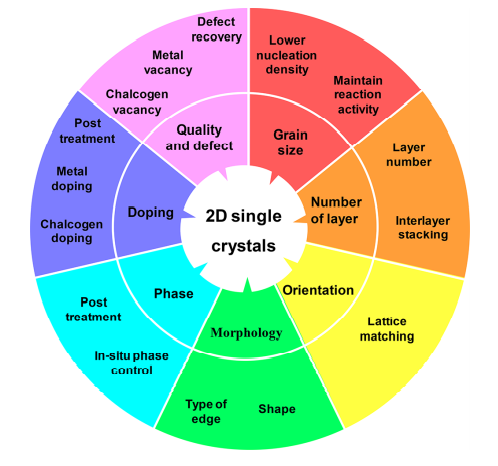
\includegraphics[scale = 0.7]{2D_material_features.PNG}
    \end{figure}
\end{frame}

\begin{frame}{Grain Size}
    \begin{itemize}
        \item Small grain -- more grain boundaries
        \item Grain boundaries -- worsen electronic, mechanical and thermal properties -- reason -- scattering of carriers, introducing more defects
        \item Practical Application -- Large area 2D materials -- large grain size
        \item Requirements -- Effective methods to grow large single crystal 2D TMDCs
        \item Currently -- submicrometer to centimeter scale 2D Materials -- \ch{MoS2}, \ch{WS2}, \ch{WSe2}, \ch{MoTe2}
        \item Strategies to increase grain size - Two
        \begin{itemize}
            \item Decrease nucleation density
            \item Maintain reaction activity for material growth for longer time
        \end{itemize}
    \end{itemize}
\end{frame}

\begin{frame}{Grain Size}
    \begin{itemize}
        \item Strategy 1 -- Decreasing the nucleation density
        \begin{itemize}
            \item Few nucleation sites -- Smooth surface -- molten glass at high temperature (Other liquid or quasi-liquid surface)
            \item Example -- \ch{MoS2} FET -- Field effect mobility of \unit{95}{\centi\meter^{2}V^{-1}s^{-1}},  on/off current ratio of $10^7$
            \item Using Additives to decrease nucleation density
            \item Example -- Oxygen introduction -- etch away unstable nuclei -- large monolayer \ch{MoS2} with domain size \unit{350}{\micro\meter} on sapphire c-plane
        \end{itemize}
        \item Strategy 2 -- Maintaining reaction activity of grain growth for longer time
        \begin{itemize}
            \item Decreasing the energy barrier for the reaction
            \item Self-limited catalytic surface growth mechanisms
            \item Examples - large area monolayer \ch{WS2} single crystal of millimeter size on Au foils, \ch{MoS2} of size \unit{80}{\micro\meter} on Au foil, \ch{WS2} of size \unit{135}{\micro\meter} on c-plane sapphire
        \end{itemize}
    \end{itemize}
\end{frame}

\begin{frame}{Grain Size}
    \begin{figure}
        \centering
        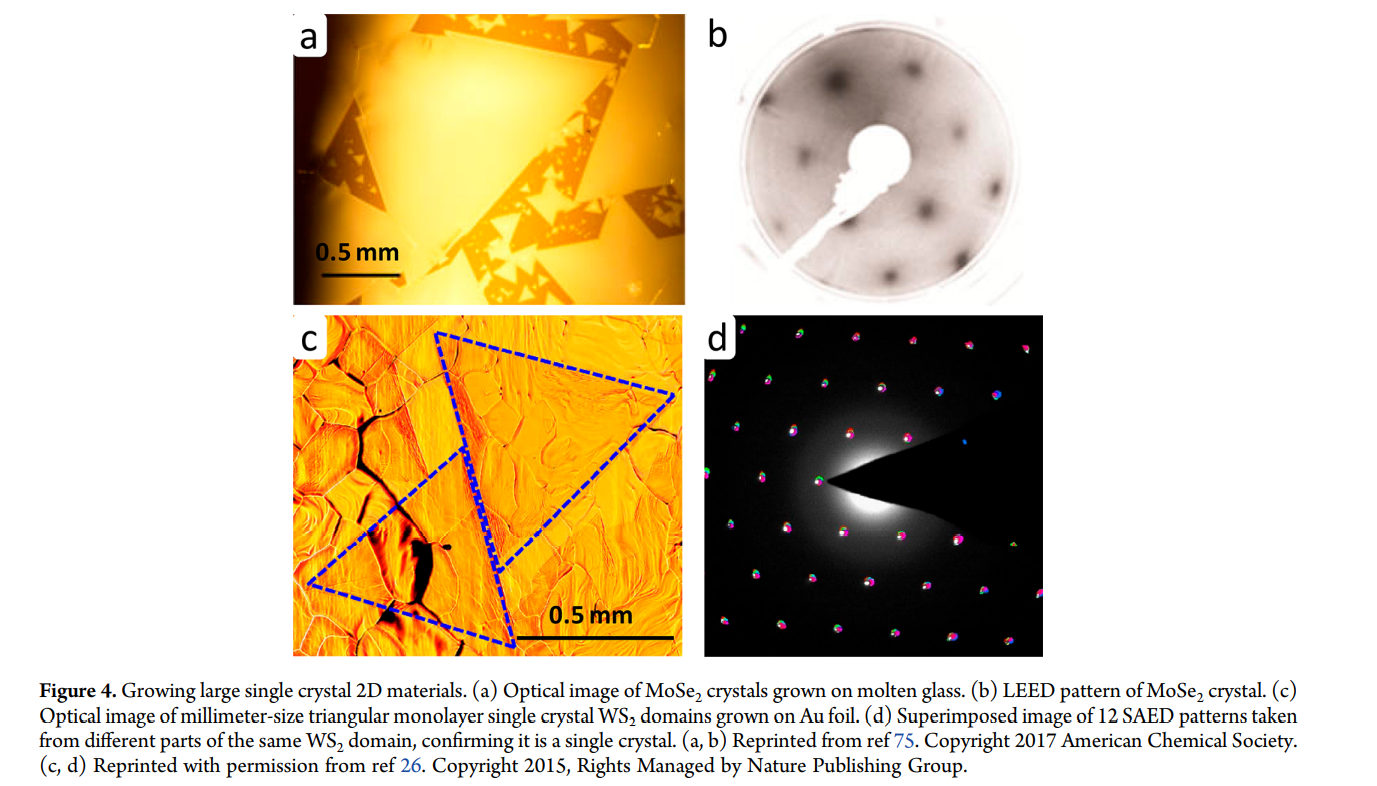
\includegraphics[scale = 0.4]{grain size.PNG}
    \end{figure}
\end{frame}

\begin{frame}{Remaining Topics to Discuss}
    \begin{itemize}
        \item Layers, Orientation, Morphology, Phase, Doping, Quality and Defects
        \item CVD growth of wafer scale continuous 2D materials films
        \item CVD growth of 2D material based heterostructure
        \item Application of CVD-grown 2D materials and their heterostructure
        \item Conclusion
        \item Epitaxial growth of 2D Layered TMDCs: Growth Mechanism, Controllability and Scalability
    \end{itemize}
\end{frame}

\begin{frame}{Descriptions}
\begin{description}
\item[CVD] Chemical Vapour Deposition
\item[TMDCs] Transition Metals Dichalcogenides
\item[PTAS] Perylene-3,4,9,10-tetracarboxylic dianhydride
\item[PTCDA] Perylene-3,4,9,10-tetracarboxylic dianhydride
\item[rGO] reduced Graphene Oxide
\item [PECVD] Plasma Enhanced CVD
\item[ICP-CVD] Inductively Coupled Plasma CVD
\item[FET] Field Effect Transistor
\end{description}
\end{frame}

\begin{frame}{References}
    \begin{thebibliography}{10}
    \bibitem[1]{Cai2018}
    Cai, Zhengyang and Liu, Bilu and Zou, Xiaolong and Cheng,Hui-Ming, Chemical Vapor Deposition Growth and Applications of Two-Dimensional Materials and Their Heterostructures, Chemical Reviews, \href{https://doi.org/10.1021/acs.chemrev.7b00536}{https://doi.org/10.1021/acs.chemrev.7b00536}
    
    \bibitem[2]{ossila} Ossila Enabling Material Science - \href{https://www.ossila.com/pages/introduction-2d-materials}{Introduction to 2D Materials}
    \bibitem[3]{wiki} \href{https://www.wikipedia.org/}{Wikipedia}
    \end{thebibliography}
\end{frame}

\begin{frame}
\begin{center}
{\fontsize{40}{50}\selectfont Thank You!}
\end{center}
\end{frame}

\end{document}
